\chapter{Introduction}

\begin{quote}
The aim of illustration is to generate expressive images that effectively convey certain information via the visual channel to the human observer.\cite{Viola-05-Smart}
\end{quote}

Illustrations have been used since the paleolithic age\cite{Viola-05-Smart} to give their viewers a graphical representation of things seen, experienced or imagined\cite{misc:WikiEnVIs}. Since the development of perspective and the necessity to intuitively explain complex technical, medical and scientific matters, especially since the industrial revolution, several techniques to successfully achieve this have been developed.
\begin{quote}
Illustrative techniques are often designed in a way that even a person with no technical understanding clearly understands the piece of art.\cite{Viola-05-Smart}
\end{quote}
With the arrival of computers that are able to create complex graphics that react in real-time to user interactions, the transfer of these static illustrations to a dynamic visual representation has posed new challenges to the art of illustration.
Exploded views are a technique used in illustrative visualization, where complex real world objects are drawn in a way that conveys how these objects are built, how they are assembled or how they work. Typically these objects are systems of interacting parts that may occlude each other or even be completely hidden by an outer hull of the visualized objects.\\
Examples for this would be a motor that consists of many independent parts, where the Illustration should give an idea of how it might work, a chest of drawers bought as a set of boards and connectors, that has a visual assembly instruction or the depiction of an anatomic feature.\\
\begin{quote}
In an exploded view the object is decomposed into several parts which are displaced so that internal details are visible \cite{proc:bruckner-2006-EVV}
\end{quote}
So for technical illustrations the parts that constitute a machine could be moved on an axis so that they are all visible and their position relative to this axis would still give information as to where the place of each part would be inside the machine. As for the assembly instruction the displacement would happen along the axes they will be put together to make it clear to the viewer how to assemble the object.\\
The goal of my work was to create an interactive visualization that would dynamically generate simple exploded views. Building upon an existing plugin for the VolumeShop visualization platform, that splits objects along a plane and displaces the two parts,  I created a plugin where the user can define an object of interest, that is not cut and stays in place, while the split parts are displaced, revealing said object.\\
The visualization system is interactive, the User can also choose, which part of the system is interesting to him, and view the object from different angles. From each perspective and foreach object of interest the system has to ensure that the object of interest is visible, the resulting visualization is compact but not too cluttered.  Because of this the ideal position of the exploded parts is constantly shifting upon interaction. To give the transitions a more natural and therefore aesthetically pleasing look this displacement- the ''explosion''- can be shown as an animation.\\
When looking from a direction close to the displacement axis, the explosion distance becomes so large, that the object of interest is either to small, because it's to far away when the whole graphic is displayed or parts of the graphic missing becuse they are behind the camera.
To prevent this, I designed a system with a maximum distance of displacement. To prevent complete occlusion I combined the exploded view with ghosting, which is a technique where Objects occluding other objects are being drawn transparently.\ref{fig:demo} \\
\begin{figure}[tb]
	\centering
	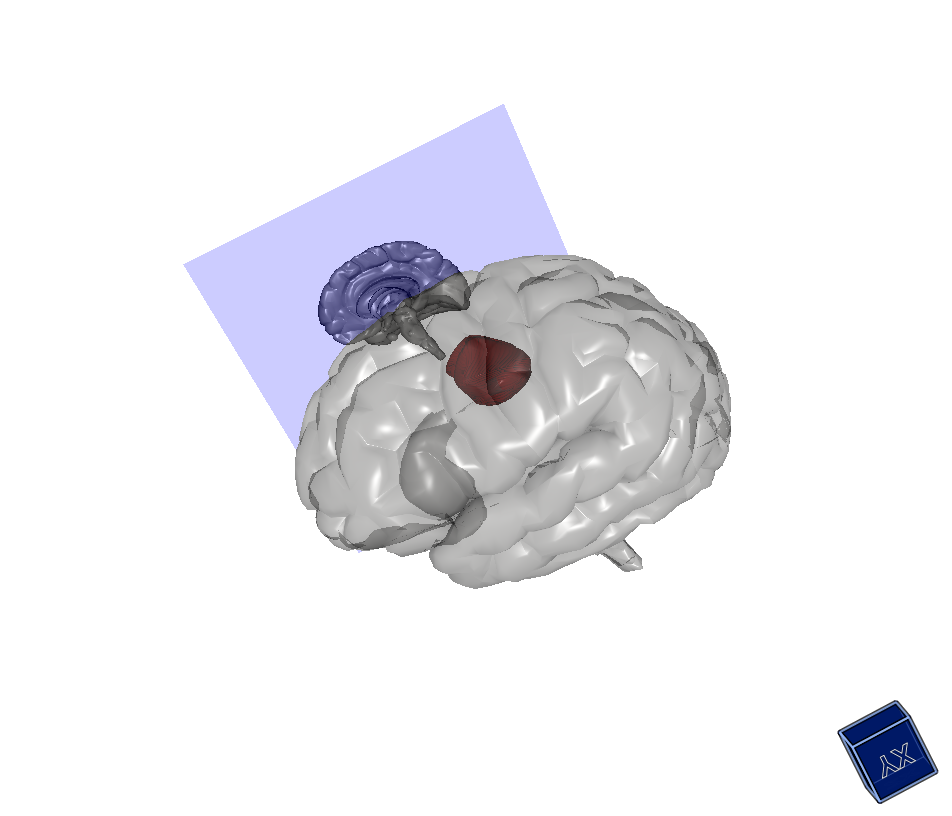
\includegraphics[width=0.7\textwidth]{chapters/figures/demo}
	\caption{Illustration of a brain, combining ghosting and an exploded view}
	\label{fig:demo}
\end{figure}